\documentclass[a4paper,oneside,article,11pt]{memoir}
\usepackage[english]{babel}
\usepackage[utf8]{inputenc}
\usepackage{amsmath,amssymb,amsthm}

% This font looks so good.
\usepackage[sc]{mathpazo}

% Typesetting pseudo-code
\usepackage{algorithm}
\usepackage{algorithmic}
\usepackage{multirow}
% Code comments like [CLRS]
\renewcommand{\algorithmiccomment}[1]{\makebox[5cm][l]{$\triangleright$ \textit{#1}}}
\usepackage{framed,graphicx,xcolor}
\usepackage[font={small,it}]{caption}
\usepackage{listings}
\usepackage{units}

% Relative references
\usepackage{varioref}

\usepackage{hyperref}
\usepackage{url}
\bibliographystyle{alpha}

\title{Range Reporting}
\author{Peter Gabrielsen 20114179 \\
Christoffer Hansen 20114637}
\newcounter{qcounter}
\begin{document}

\begin{titlingpage}
\clearpage

\maketitle
\thispagestyle{empty}

\begin{abstract}
blabla
\end{abstract}
\end{titlingpage}

\pagebreak

\tableofcontents

\pagebreak

\chapter{Introduction}
\label{chp:introduction}
% words: big data, banking, data larger than memory, database community, slow disks, disparity between growth of CPU speeds and transfer speeds between internal and external memory (widening gap)
% fault tolerance and consistency are more challenging to handle in-memory (In-Memory Big Data Management and Processing: A survey)
% storage prices
% The I/O bottleneck
% Disk were faster than CPU in 60
% http://read.cs.ucla.edu/111/2006fall/notes/lec15#incommensurate-scaling

In the early days of computers disks were faster than processors. Since then processor technology has advanced at an incredible rate achieving annual speedups of 40 to 60 percent~\cite{ruemmler_wilkes_1994}. Although this is also true for disk capacity an entirely different story can be told for the speedup of disk performance. The disparity between processor, internal memory, and external memory speeds have grown larger for each year and the gap is widening. This disparity presents serious problems when designing algorithms on large data sets, and with more and more applications of Big Data in social media, banking, etc., these problems become increasingly relevant.

%TODO get a better figure. This one is really ugly.
\begin{figure}[h]
	\centering
		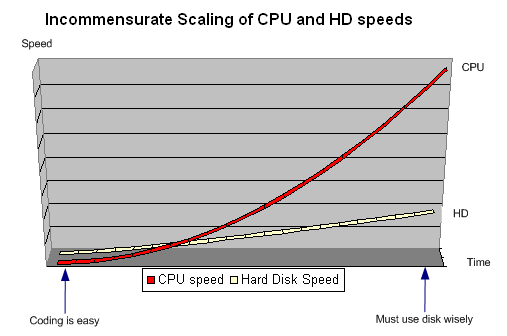
\includegraphics[scale=0.5]{../figures/scaling-of-cpu-vs-disk}
	\caption{Growth of CPU compared to HD speeds over time.}
	\tiny{Source:~\protect\url{http://read.cs.ucla.edu/111/2006fall/notes/lec15\#incommensurate-scaling}}
	\label{fig:cpu_vs_disk}
\end{figure}

While the database community has always been involved in development of practically efficient external memory data structures, most algorithms research has focused on worst-case efficient internal memory data structures. With the advent of Big Data and problems concerning large data sets the algorithms community has been increasingly involved in developing worst-case efficient external memory data structures for solving these problems~\cite{ionote}.

To some large internet companies the bottleneck that disk-based systems presents has become to great of an obstacle and in an attempt to close the gap they have moved towards developing internal memory big data processing. This move has been allowed by growing main memory capacities but it comes with the price of issues such as fault-tolerance and consistency which are inherently more challenging to handle in volatile memory~\cite{Zhang2015}.

Another price of this move to internal memory is the actual cost of running server farms and the cost of internal memory compared to external memory. The extra costs and increased complexity suggests that external memory data structures have some well defined advantages.

In disk-based systems algorithms and data structures cannot be measured in the traditional models used for internal memory algorithms since the performance is bound by disk latency. In Section~\ref{chp:iomodel} we investigate a model that encapsulates performance of the I/O bottleneck.

In Section~\ref{chp:prelims} we give a preliminary overview of some of the techniques used in developing external memory efficient data structures.

%TODO add more sections!

\chapter{Model of computation}
\label{chp:iomodel}
We will argue the results of this thesis in terms of the external memory model of Aggarwal and Vitter~\cite{Aggarwal:1988/ICS/48529.48535}.
The external memory model (or I/O model) measures the efficiency of an algorithm by counting the total number of reads and writes performed. In detail the model consists of two levels of memory; a bounded internal memory of size $M$ and an unbounded external memory. For a total of $N$ records we define an \textit{IO} operation to the process of transferring $B$ consecutive records between the two levels of memory as depicted in figure~\ref{fig:io_model}. We restrict all computations on records to be done in internal memory. Throughout the thesis we will let $K$ denote the total number of records in the output.


\begin{figure}[h]
	\centering
	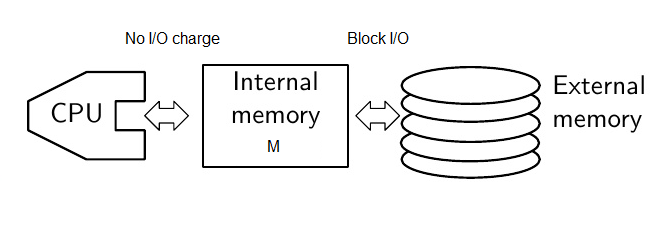
\includegraphics[width=0.8\textwidth]{../figures/io_model.png}
	\caption{The IO Model. Only reads/writes between internal and external memory is charged.}
	\label{fig:io_model}
\end{figure}

The fundamental bounds in the external memory model is that scanning can be done in $\mathcal{O}(\text{Scan}) = \mathcal{O}(\nicefrac{N}{B})$, sorting in $\mathcal{O}(\text{Sort}) = \mathcal{O}(\nicefrac{N}{B} \log_{\nicefrac{M}{B}}\nicefrac{N}{B})$ and searching in $\mathcal{O}(\log_B N)$. We denote $\mathcal{O}(\nicefrac{N}{B})$ as being linear in terms of IOs. Note that the $B$ factor is very important as $\nicefrac{N}{B} < \mathcal{O}(\nicefrac{N}{B} \log_{\nicefrac{M}{B}}\nicefrac{N}{B}) \ll N$.

For convenience we will assume $M > B^2$. This assumption is known as the \textit{tall-cache assumption} in the cache-oblivious model and basically states that the number of blocks \nicefrac{M}{B} is larger than the size of each block $B$~\cite{Prokop99cache-obliviousalgorithms}.

\chapter{Preliminaries}
\label{chp:prelims}
% amortization

\section{Amortization}

\section{Global rebuilding}
The term \textit{global rebuilding} refers to the standard technique of making a (typically small) static data structure dynamic. We simply store all updates in a \textit{update block} and once a certain threshold has been collected we rebuild the data structure~\cite{ionotes}. For data structures that does not allow the space for deleted records to be reoccupied we \textit{mark} (or \textit{weak delete}) the elements. Whenever $\alpha N$ elements have been marked, for some constant $\alpha > 0$, the entire data structure is rebuilt from scratch with only the non-marked elements. The cost of rebuilding is at most a constant factor higher than the cost of inserting $\alpha N$ elements and so the amortized cost of global rebuilding can be charged to the insertions of the deleted elements~\cite{Meyer:2003/AMH/1744652}.

\section{Filtering}
The techinque 

Charge part of query cost to output.

\chapter{Sublogarithmic Updates}

\chapter{External Memory Priority Search Tree}

\bibliography{references}

\end{document}


